\chapter{1. A construção da integração mundial}

\coment{Este módulo foi estruturado seguindo uma linha temporal que explicita o
desenvolvimento do processo de globalização e, ao mesmo tempo, mobiliza
os conteúdos necessários para a efetivação do eixo e das habilidades
associadas.\\
Habilidades da BNCC: EF09GE05, EF09GE06, EF09GE09.}

\colorsec{Eixo de conhecimento do SAEB}

\begin{itemize}
\item Tempo e espaço: fontes e formas de representação
\end{itemize}

\conteudo{O desenvolvimento da configuração de mundo atual é resultado de longo processo histórico, que não pode ser compreendido sem considerarmos o papel da colonização e do desenvolvimento do capitalismo, sistema econômico que hoje integra todo o mundo em sua lógica.

Tal processo possui íntima relação com o desenvolvimento da cartografia, que, desde suas bases na Antiguidade, desenvolveu-se seguindo os rumos das grandes navegações, o que torna evidente também quanto a Antiguidade Clássica relaciona-se com a Europa que colonizou o mundo.

A globalização integrou o mundo por meio do desenvolvimento tecnológico e da consolidação do capitalismo a nível global, conseguindo estabelecer padrões gerais de consumo, cultura e organização social. Tal interação assenta-se no predomínio das lógicas ocidentais do mundo gestadas na Europa.}

\coment{Ao longo das atividades, ficará perceptível que as questões estão
encadeadas, de modo que o conteúdo vai se
articulando por meio de atividades interpretativas que mobilizam também o
conteúdo previsto para ser visto ao longo dos quatro Anos Finais do Ensino
Fundamental. Essa é uma forma que facilita a compreensão
do aluno ao seguir uma estrutura que remete a uma sequência de aulas.}


\colorsec{Atividades}

\begin{quote}
Os mapas medievais "T e O" originaram-se da descrição do mundo na
obra \emph{Etymologia}, de Isidoro de Sevilha. Este conceito de
cartografia medieval representa apenas o hemisfério norte de uma Terra
esférica, dedução feita a partir da projeção da porção habitada do mundo
conhecida nos tempos romanos e medievais.

\begin{figure}[htpb!]
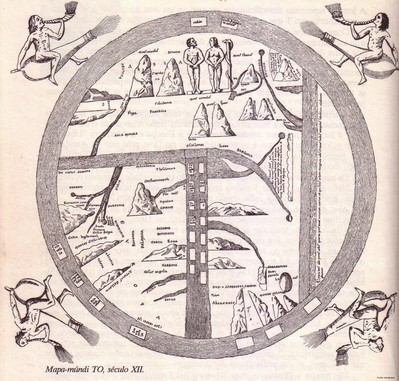
\includegraphics[width=2.88577in,height=2.76032in]{./imgs/img1.jpg}
\caption{Fonte: /www.geografia.seed.pr.gov.br/modules/galeria/detalhe.php?foto=401\&evento}
\end{figure}

O "T" é o Mediterrâneo
dividindo em três contimentes: Europa, Ásia e África, sendo o "O" um
Oceano circundante. Jerusalém era usualmente representada no centro do
mapa e a Ásia surgia do tamanho da soma dos outros dois continentes.
Porque o Sol nascia a leste, e o Paraíso (jardim do Éden) era geralmente
representado como sendo na Ásia, estando, dessa maneira, situada na
porção superior do mapa.

\fonte{Secretaria da Educação. Mapa T O. Disponível em: \emph{www.geografia.seed.pr.gov.br/modules/galeria/detalhe.php?foto=401\&evento}. Acesso em: 19 fev. 2023.}
\end{quote}

\num{1} Mapas são representações não apenas do espaço geográfico, mas também
de ideias e concepções de mundo. No caso do mapa T O, qual era a
concepção de mundo em sua base?

\linhas{4}

\coment{Como o mapa representava apenas a porção do planeta conhecida pelos
elaboradores, a concepção de mundo deles acreditava que não existia mais
superfície terrestre para além das áreas conhecidas, sendo esse conjunto
o único tipo de mundo aceito como existente.}

\num{2} O mapa T O era um mapa medieval, de uma época em que não estavam prontas as
bases da cartografia como a conhecemos hoje. Circule os nomes dos elementos que estão ausentes nesse mapa, mas que devem
\textbf{obrigatoriamente} existir nos mapas contemporâneos.

\begin{multicols}{2}
\red{LEGENDA}

FIGURAS

\red{TÍTULO}

SIMBÓLICAS

TRAÇADO DE ESTRADAS
\end{multicols}

\coment{Os mapas contemporâneos precisam dispor de alguns elementos básicos,
como título, legenda, escala e orientação. Esses elementos permitem
identificarmos o tema, como ele está sendo representado, comparação
entre o tamanho do mapa e o tamanho da área representada e a disposição
dos elementos espaciais no espaço.}

\num{3} Leia os dois textos a seguir.

\textbf{TEXTO 1}
\begin{quote}

{[}...{]}

Durante muitos séculos, os mapas foram um privilégio da elite.
Apenas reis, nobres, alto clero, grandes navegadores e armadores de
expedições marítimas, tinham acesso a esse tipo de informação. Somente a
partir da invenção da imprensa, na segunda metade do século XV, os mapas
puderam ser mais amplamente utilizados.

{[}...{]}

\fonte{IBGE. \emph{Atlas Geográfico Escolar na
Internet.} Disponível em:
\emph{https://atlasescolar.ibge.gov.br/conceitos-gerais/historia-da-cartografia/a-era-dos-descobrimentos-sec-xv-a-xviii.html}.
Acesso em: 19 fev. 2023.}
\end{quote}

\textbf{TEXTO 2}
\begin{quote}

Depois de inventar os tipos móveis, Gutenberg ajudou a dar início
a uma revolução cultural. Os padrões de impressão definidos por ele
consolidaram-se de tal forma que se mantiverem sem grandes alterações
até o século XVIII. Por isso, o nome de Gutenberg está na lista dos
personagens mais influentes da história. Em 2000, por exemplo, alguns
meios de comunicação o definiram como o \textbf{homem do milênio}.

\fonte{Fonte de pesquisa: National Geographic Portugal. Johannes Gutenberg e os princípios da impressão. Disponível
em: \emph{https://nationalgeographic.pt/historia/grandes-reportagens/3086-johannes-gutenberg-e-os-principios-da-impressao}.
Acesso em: 19 fev. 2023.}
\end{quote}

Agora, leia esta afirmativa:

\textit{A popularização e o aperfeiçoamento dos mapas estão diretamente relacionados
ao avanço técnico ocorrido às vésperas do mercantilismo.}

Explique se você concorda com essa afirmativa ou se você discorda dela.

\linhas{4}

\coment{A articulação entre os textos deixa claro que os mapas deixaram de ser
privilégio da elite apenas após a capacidade de impressão em massa dos
mapas ser atingida, ou seja, temos uma inovação técnica associada ao
desenvolvimento cartográfico.}

\num{4} Leia o texto.

\begin{quote}
\textbf{Mercantilismo}

{[}...{]}

A obtenção de riqueza no mercantilismo poderia se dar de diversas
maneiras. O Estado poderia cobrar impostos da população, vender cargos
públicos e títulos de nobreza, confiscar bens, ceder privilégios
comerciais para um determinado grupo em troca de compensação financeira
(monopólios), exportar mercadorias, saquear em contextos de guerra,
cobrar taxas alfandegárias, realizar ações de pirataria
etc.

{[}...{]}

Um acontecimento extremamente importante para o sucesso
dessas práticas econômicas entre as nações europeias foi o
colonialismo.

O colonialismo foi fundamental para os Estados europeus, pois
permitiu que eles explorassem inúmeros recursos de suas colônias e os
enviassem para a Europa. Isso também possibilitou que essas colônias
fossem transformadas em consumidores compulsórios de suas metrópoles,
por conta do exclusivismo comercial.

{[}...{]}

\fonte{Daniel Neves Silva. História do Mundo. Mercantilismo. Disponível em:
\emph{https://www.historiadomundo.com.br/idade-moderna/mercantilismo.htm}.
Acesso em: 19 fev. 2023.}
\end{quote}

Na Idade Média, considerava-se o mundo como
restrito a Europa, Ásia e África. A partir da leitura do texto, o que
muda na visão europeia sobre a extensão do mundo a partir do
mercantilismo?

\linhas{4}

\coment{Em contraposição à ideia de um mundo restrito a Ásia, Europa e África, a
colonização marcou também a ``descoberta'' do continente americano pelos
europeus, o que ampliou o mundo conhecido até então.}

\num{5} A globalização é caracterizada pela integração de fluxos comerciais,
populacionais, culturais e sociais. Como a imagem abaixo relaciona-se
com a globalização?

\linhas{5}

\begin{figure}[htpb!]
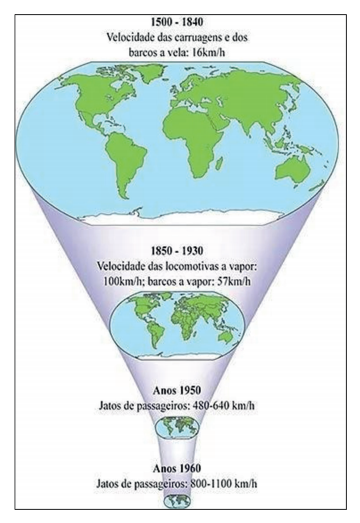
\includegraphics[width=2.70776in,height=3.93646in]{./imgs/img2.png}
\caption{Fonte: Harvey, D. A condição pós-moderna. 16 ed. São Paulo: edições Loyola, 2007. p. 220}
\end{figure}

\coment{A imagem é um conjunto de representações cartográficas que diminuem a
medida que os meios de transporte se desenvolvem, relacionando assim a
diminuição de distâncias a redução do tamanho do mundo, que seria a
maior rapidez nos deslocamentos de pessoas e mercadorias, característica
da globalização.}

\num{7}

\begin{quote}
A origem dos termos \emph{sociedade global}
e \emph{globalização} é anterior ao triunfo político
da \emph{globalização} neoliberal; data
de finais dos anos 1960 e deve ser creditada a MacLuhan e a Bzezinski
{[}...{]} Brzezinski colocou em circulação as expressões cidade global e
sociedade global para designar a nova reconfiguração globalizada do
nosso habitat, operada pelas redes tecnotrônicas termo introduzido por
ele para designar a conjugação do computador, da TV e da rede de
telecomunicação. O protótipo dessa `sociedade global' eram os EE.UU.,
centro propulsor da revolução `tecnotrônica' mundial que oferecia ao
mundo o `único modelo global de modernidade', com os correspondentes
`padrões de comportamento e valores universais'.

\fonte{CASTRO, Ramon Peña. \emph{Dicionário da
Educação Profissional em Saúde.} Disponível em:
http://www.sites.epsjv.fiocruz.br/dicionario/verbetes/glo.html.
Acesso em: 19 fev. 2023.}
\end{quote}

Segundo o texto, como o advento de novas tecnologias de comunicação
ajudou a integrar o conjunto dos países?

\linhas{5}

\coment{Os meios de comunicação tornam possível a transmissão de informações
para lugares distantes, não apenas informação, mas também ideias,
modelos de vida e manifestações culturais. Quem domina os meios de
comunicação também domina o que é transmitido, ajudando a moldar os
discursos dominantes.}

\num{8}

\begin{quote}
\textbf{Saiba um pouco mais sobre a história do movimento Manguebeat}

O manguebeat surgiu em Pernambuco,como um movimento de
contracultura. Ele era formado principalmente por jovens que usavam a
música como uma forma de inclusão social {[}..{]}.

O nome surgiu de uma fusão da palavra mangue com a palavra bit
(unidade de memória de computadores). Assim como o mangue, que é rico em
sua biodiversidade, o manguebeat criou uma cena musical bem
diversificada, misturando ritmos regionais pernambucanos como: maracatu,
frevo, ciranda e caboclinho, pop, rap, hip hop e música eletrônica. O
movimento se beneficiou de ferramentas tecnológicas recém surgidas, o
quê proporcionou a gravação das músicas em ``home studios'' e do
surgimento da internet, principal fonte de divulgação.

Diversos grupos se destacaram: Mundo Livre S/A, Chico Science \&
Nação Zumbi, Sheik Tosado, Mestre Ambrósio, Faces do Subúrbio, Eddie,
Via Sat, Querosene Jacaré e Jorge Cabeleira.

\fonte{Disponível em: https://tv.unesp.br/old/616. Acesso
em: 19 fev. 2023.}
\end{quote}

Músicas como pop, rap e eletrônica possuem origem diversas para além das
fronteiras brasileiras, nesse sentido, o que a mistura desses ritmos por
grupos brasileiros pode nos dizer sobre a globalização?

\linhas{5}

\coment{A fusão de ritmos demonstra que a música não se restringe mais aos
países e territórios onde são criadas, espalhando-se através dos meios
de comunicação, o que permite também a apropriação por outros grupos,
isso gera uma integração cultural característica da globalização.}

\num{9} Leia as informações abaixo:

\paragraph{I} Veja abaixo quais foram os 10 produtos mais exportados pelo Brasil em
2022, segundo informações do ComexStat.

\begin{enumerate}
\item \salmao{Soja}
\item \salmao{Minério de ferro} e seus
\item Óleos brutos de \salmao{Petróleo}
\item \salmao{Açúcares} e melaços
\item \salmao{Carne bovina}
\item \salmao{Farelos de Soja} e outros alimentos para animais (excluídos cereais não
  moídos), farinhas de carnes e outros animais
\item \salmao{Celulose}
\item \salmao{Milho} não moído, exceto milho doce
\item Demais produtos -- \salmao{indústria da transformação}
\item \salmao{Carnes de aves} e suas miudezas comestíveis, frescas, refrigeradas ou congeladas
\end{enumerate}

\fonte{SPRENGER, Leandro. Principais Produtos
Exportados para China. Disponível em:
https://www.fazcomex.com.br/comexstat/asia/exportacao-china/. Acesso em:
22 fev. 2023.}

\paragraph{II} Confira a lista dos principais produtos que o Brasil importa da China.

\begin{enumerate}
\item
  Equipamentos de telecomunicações
\item
  Válvulas e tubos termiônicas
\item
  Compostos organo-inorgânicos
\item
  Demais produtos - Indústria de Transformação
\item
  Adubos ou fertilizantes
\item
  Medicamentos e produtos farmacêuticos, exceto veterinários
\item
  Máquinas e aparelhos elétricos
\item
  Peças e acessórios para escritório
\item
  Aparelhos elétricos para ligação
\item
  Máquinas de energia elétrica
\end{enumerate}

\fonte{SPRENGER, Leandro. Principais Produtos
Importados da China. Disponível em:
https://www.fazcomex.com.br/comex/produtos-importados-da-china-para-o-brasil/}

\num{a)} Quem vende mais produtos industrializados, Brasil ou China? O que
isso revela sobre a relação entre os dois países?

\linhas{2}

\coment{A China vende mais produtos industrializados do que o Brasil, isso
mostra que o parque industrial chinês e mais desenvolvido, e que a
indústria tem menor participação na composição econômica do Brasil.}

\num{b)} A produção industrial mundial concentra-se na América do Norte, leste
da Ásia e oeste da Europa, a partir dessa constatação, analise a
afirmativa a seguir:

\begin{quote}
A globalização é marcada por um pequeno grupo de países produtores e um
imenso grupo de consumidores.
\end{quote}

Explique o significado desta afirmativa.

\linhas{3}

\coment{A tabela mostra que a produção industrial é concentrada, isso mostra que
a produção industrial é monopólio de poucos países, ou seja, eles
produzem aquilo de mais avançado existente até hoje, enquanto o restante
do mundo apenas consome os produtos e reproduzem a tecnologia fabril
oriunda de outros países.}

\colorsec{Treino}

\num{1} 

\begin{quote}
De modo geral, podemos definir o mundo oriental como a porção
da Terra formada pelas nações da Ásia e do Oriente Médio, enquanto o
mundo ocidental engloba a Europa e grande parte dos territórios que
foram colonizados pelos europeus, notadamente a América, a Austrália e a
Nova Zelândia. {[}...{]}

\fonte{Disponível em:
https://sme.goiania.go.gov.br/conexaoescola/eaja/geografia-mundo-oriental-e-mundo-ocidental/.
Acesso em: 20 fev 2023.}
\end{quote}

Identifica-se no texto que o mundo ocidental corresponde

\begin{escolha}
\item
  ao conjunto dos países europeus.
\item
  as sociedades que seguem o islamismo.
\item
  aos territórios localizados no hemisfério oeste.
\item
  aos países condicionados pela cultura europeia.
\end{escolha}

\coment{SAEB: Considera o campo instrumental e metodológico da Geografia e da
História, abarcando aprendizagens relativas a categorias como as de
continuidades, mudanças e rupturas, bem como habilidades de
identificação, análise, descrição, comparação e construção de
explicações sobre espaços e tempos em relações multiescalares (local,
regional, nacional e global).

BNCC: (EF09GE06) Associar o critério de divisão do mundo em Ocidente e
Oriente com o Sistema Colonial implantado pelas potências europeias.

a) Incorreta. No texto consta que a porção colonizada pela Europa também
  integra o mundo ocidental; b) Incorreta: O Islamismo é uma religião presente majoritariamente no
  mundo oriental; c) Incorreta. Essa concepção considera apenas a posição dos países no
  globo, mas a concepção de mundo ocidental considera principalmente o
  aspecto cultural; d) Correta. O mundo ocidental é entendido como o conjunto dos países e
  sociedades que foram condicionados em alguma medida pela sociedade
  europeia ocidental, isso inclui a própria Europa e todo o conjunto de
  países colonizados pelos europeus, como o continente americano,
  Austrália e Nova Zelândia.}

\num{2} 

\begin{quote}
Isodoro (570-636 d.C.), bispo de Sevilha, criou o mapa
etimologias, também conhecido como mapa T-0. Este mapa esquemático tinha
o seguinte significado: o "T" representava os três cursos d'água que
dividiam o ecúmero, o Mediterrâneo, que separa a Europa da África; o
Nilo, separando a África da Ásia; e o Don, entre a Ásia e a Europa. O
ecúmero teria sido dividido por Noé entre seus três filhos após o
Dilúvio. Além disso, o "T" também simbolizava a cruz e na sua junção
estaria localizada Jerusalém, centro do mundo. Esses mapas, em sua
maioria, eram circulares e emoldurados por um grande oceano.

\fonte{IBGE. \emph{Atlas Geográfico Escolar na
Internet.} Disponível em:
https://atlasescolar.ibge.gov.br/conceitos-gerais/historia-da-cartografia/a-idade-media.html.
Acesso em: 20 fev. 2023.}
\end{quote}

A concepção de um mundo restrito a Europa, Ásia e África representada
nos mapas T-O explica-se pelo(a)

\begin{escolha}
\item
  restrito conhecimento astronômico.
\item
  inexistência de satélites que fotografassem do espaço.
\item
  desconhecimento de outros locais por parte dos europeus.
\item
  crença de existência em um mundo habitado por seres míticos.
\end{escolha}

\coment{SAEB: Contempla ainda o conhecimento necessário para identificação e
compreensão dos diversos elementos que compõem a cartografia.

BNCC: (EF09GE05) Analisar fatos e situações para compreender a
integração mundial (econômica, política e cultural), comparando as
diferentes interpretações: globalização e mundialização.

a) Incorreta. A astronomia é uma ciência que se desenvolve desde o Egito
  e a Grécia antiga; b) Incorreta. Os primeiros mapas não dependiam de satélites para sua
  confecção, se baseavam em dados de navegação, esquemas matemáticos
  idealizações do mundo; c) Correta. O mapa T-O representava apenas a porção do mundo conhecida
  por seus elaboradores, assim, todo o continente americano ficava de
  fora desta representação, pois apenas o mundo conhecido era
  representado; d) Incorreta. Apesar da existência de lendas sobre a existência de seres
  míticos para além do mundo conhecido, essas lendas só aparecerão mais
  fortemente durante as grandes navegações.}

\num{3}

\begin{quote}
Conforme define sua Carta de Princípios, o Fórum Social Mundial
é um espaço internacional para a reflexão e organização de todos os que
se contrapõem à globalização neoliberal e estão construindo alternativas
para favorecer o desenvolvimento humano e buscar a superação da
dominação dos mercados em cada país e nas relações internacionais.
{[}...{]}

\fonte{Disponível em:
http://forumsocialportoalegre.org.br/forum-social-mundial/. Acesso
em: 20 fev.2023.}
\end{quote}

A justificativa apresentada pelo texto valida a ideia de que a
globalização seria um sistema mundial baseado

\begin{escolha}
\item
  na integração dos sistemas políticos nacionais.
\item
  na solidariedade mútua entre a comunidade global.
\item
  no desenvolvimento pleno dos antigos países colonizados.
\item
  no domínio territorial por parte dos mercados desenvolvidos.
\end{escolha}

\coment{SAEB: Aborda as articulações entre tempo e espaço, contemplando o
trabalho com as diversas fontes históricas e geográficas, de forma que
possibilite a interpretação e a leitura crítica, a partir da diversidade
de linguagens e meios disponíveis de documentação e registro.

BNCC: (EF09GE05) Analisar fatos e situações para compreender a
integração mundial (econômica, política e cultural), comparando as
diferentes interpretações: globalização e mundialização.

a) Incorreta. Não existe no texto a contraposição a ideia apresentada
  pela alternativa; b) Incorreta. Não existe no texto a contraposição a ideia apresentada
  pela alternativa, além disso, a menção a busca pelo desenvolvimento
  humano e a crítica ao neoliberalismo evidenciam que o fórum critica a
  falta dos aspectos apresentados na alternativa; c) Incorreta. O fato de se reivindicar maior desenvolvimento humano é uma
  evidência que atesta o não desenvolvimento dos países
  subdesenvolvidos; d) Correta. No texto se critica a política neoliberal, ou seja, aquela
  que coloca nos mercados e empresas financeiras o centro das políticas
  econômicas, permitindo que o capital financeiro de países estrangeiros
  possa agir sem regulamentação em todo o mundo.}

\chapter{SIMULADO}

\num{1} Observe a imagem abaixo:

\begin{figure}[htpb!]

\includegraphics[width=2.57295in,height=1.68827in]{./imgs/img3.jpg}
\caption{Fonte: https://pt.wikipedia.org/wiki/Arado\#/media/Ficheiro:Maler\_der\_Grabkammer\_des\_Sennudem\_001.jpg. Antigo arado egípcio, circa 1200 a.C}
\end{figure}

No contexto apresentado, o arado cumpria a função de

\begin{escolha}
\item
  otimizar o trabalho humano.
\item
  domesticar os animais.
\item
  criar redes de água
\item
  limpar terrenos.
\end{escolha}

\coment{SAEB: Aborda as articulações
entre tempo e espaço, contemplando o trabalho com as diversas fontes
históricas e geográficas, de forma que possibilite a interpretação e a
leitura crítica, a partir da diversidade de linguagens e meios
disponíveis de documentação e registro.

BNCC: (EF09GE05) Analisar fatos e situações para compreender a
integração mundial (econômica, política e cultural), comparando as
diferentes interpretações: globalização e mundialização.

a) Correta. O arado está sendo utilizado para diminuir o tempo gasto com
preparo e semeadura do solo, sendo assim, constitui um instrumento que
otimiza o trabalho humano, isto é, a transformação de recursos naturais
em produtos com valor de uso; b) Incorreta. Não se evidencia na imagem a utilização do arado para
domesticação, o fato de bois estarem o puxando quer dizer que eles já
são domesticados;
c) Incorreta. O arado é um instrumento de preparação do solo para plantio;
d) Incorreta. O arado é empregado em terrenos já disponibilizados ao
plantio.}

\num{2}

\begin{quote}
\textbf{Texto I}

A indústria brasileira dá sinais de que algo de errado acontece no
setor. Do início do ano até agora, três gigantes multinacionais
anunciaram que vão abandonar o Brasil. A norte-americana Ford deixa o
mercado de fabricação de veículos nacional depois de mais de 100 anos. A
alemã Mercedes-Benz fecha a única fábrica no Brasil de carros de luxo. A
japonesa Sony fecha a fábrica em Manaus (AM) e abandona o mercado de
televisores, câmeras e aparelhos de áudio. Esse movimento mostra que o
País passa por um processo de desindustrialização, e não é de hoje, como
sugerem alguns números e apontam especialistas.

\fonte{Ferraz Jr. Processo de desindustrialização no Brasil se
acentua. In: \emph{Jornal da Usp}. 04 mar.2021.Disponível em:
https://jornal.usp.br/atualidades/processo-de-desindustrializacao-no-brasil-se-acentua/.
Acesso em: 22 fev. 2023.}
\end{quote}

\begin{quote}
\textbf{Texto II}

As exportações do agronegócio alcançaram valores recordes para o
mês de dezembro passado e também para o ano de 2021. Foram US\$ 9,88
bilhões, valor recorde para os meses de dezembro: 36,5\% superior aos
US\$ 7,24 bilhões de 2020. Em 2021, o total exportado com o agronegócio
resultou em US\$ 120,59 bilhões, alta de 19,7\%, em relação ao ano
anterior, conforme dados divulgados nesta quinta-feira (13) pela
Secretaria de Comércio e Relações Internacionais (SCRI) do Ministério da
Agricultura, Pecuária e Abastecimento (Mapa).

\fonte{Disponível em: www.gov.br/agricultura/pt-br/assuntos/noticias/exportacoes-do-agronegocio-batem-recorde-em-dezembro-e-no-ano-de-2021. Acesso em: 22 fev. 2023.}
\end{quote}

Associando-se os textos, é possível diagnosticar que no contexto
globalizado atual o Brasil tem se constituído como

\begin{escolha}
\item
  exportador de serviços e consumidor de \emph{commodities.}
\item
  investidor tecnológico e consumidor de industrializados.
\item
  exportador de produtos básicos e consumidor de tecnologia.
\item
  centralizador da indústria global e exportador de produtos básicos.
\end{escolha}

\coment{SAEB: Considera o campo instrumental e metodológico da Geografia e da
História, abarcando aprendizagens relativas a categorias como as de
continuidades, mudanças e rupturas, bem como habilidades de
identificação, análise, descrição, comparação e construção de
explicações sobre espaços e tempos em relações multiescalares (local,
regional, nacional e global).

BNCC: (EF09GE05) Analisar fatos e situações para compreender a
integração mundial (econômica, política e cultural), comparando as
diferentes interpretações: globalização e mundialização.

a) Incorreta. O setor de serviços constitui destaque interno no Brasil,
  ele vale para a produção de \emph{commodities};
b) Incorreta. A desindustrialização demonstra que o Brasil passa por um
  processo de perda de tecnologia, seja por perder empresas detentoras
  de tecnologias, seja por não investir na tecnologia, setor que anda
  lado a lado com o desenvolvimento industrial;
c) Correta. O recorde de exportações agrícolas revela o pleno
  desenvolvimento do setor no país, o que mostrar que o Brasil tem se
  especializado na produção de itens básicos classificados como
  matéria-prima \emph{(commodities)}, essa configuração econômica
  contribui para o país ficar dependente de tecnologia externa já que o
  desenvolvimento tecnológico, mesmo para máquinas agrícolas, parte do
  setor industrial;
d) Incorreta. Já que é mencionado a perda crônica de empresas
  industriais.}

\num{3} 

\begin{quote}
Com o primitivismo característico do homem europeu culto e
nobre do século XVI, o cronista português Pero de Magalhães Gândavo
diagnosticou o que a seu ver seria a mácula original do caráter do
silvícola brasileiro. Depois de uma viagem ao Brasil em 1570, ele
escreveu que os índios não podiam ser mesmo grande coisa, pois na língua
deles "não se acham F, nem L, nem R, coisa digna de espanto, porque
assim não têm Fé, nem Lei, nem Rei". A confusão mental de Gândavo, que
não via ordem ou justiça possíveis em uma sociedade estranha se ela não
reproduzisse fielmente os vocábulos de seu próprio idioma, não difere
muito da imagem que seus contemporâneos tiveram dos índios. Cinco
séculos depois, essa imagem praticamente se inverteu. Os índios são
idolatrados. No Brasil do século XXI, todo dia é dia de índio. Os
selvagens são vistos como defensores da floresta e guardiães de culturas
e línguas que precisam ser preservadas a todo custo. {[}...{]}

\fonte{Agência Estado. Mineração em Terras Indígenas. In:
\emph{Veja,} 28 abr. 2004,p.48-50. Disponível em:
https://terrasindigenas.org.br/noticia/30695. Acesso em: 22 fev. 2023.}
\end{quote}

A fala de Pero Magalhães é um demonstrativo de que a sociedade tida como
correta, em sua visão, teria como base

\begin{escolha}
\item
  a ausência da figura do rei.
\item
  a adoção da língua portuguesa.
\item
  a ideia de proteção ambiental dos indígenas.
\item
  as características políticas e sociais do leste europeu.
\end{escolha}

\coment{SAEB: Aborda as articulações entre tempo e espaço, contemplando o
trabalho com as diversas fontes históricas e geográficas, de forma que
possibilite a interpretação e a leitura crítica, a partir da diversidade
de linguagens e meios disponíveis de documentação e registro.

BNCC: (EF09GE06) Associar o critério de divisão do mundo em Ocidente e
Oriente com o Sistema Colonial implantado pelas potências europeias.

a) Incorreta. Não apenas a ausência da figura do monarca é criticada, mas
também a ausência da fé cristã e da lei europeia;
b) Incorreta.O centro da visão colonialista não estava na língua falada,
mas nas características culturais diferenciadas dos povos indígenas;
c) Incorreta. No texto, tal ideia é tida como valorosa atualmente, não
aparecendo na fala de Pero Magalhães reproduzida;
d) Correta. A monarquia, a fé cristã com status de instituição de estado e
a legislação portuguesa são encaradas como base de uma civilização
correta na fala de Pero Magalhães, por isso ele critica a ausência
desses elementos entre os indígenas.}

\num{4} 

\begin{figure}[htpb!]
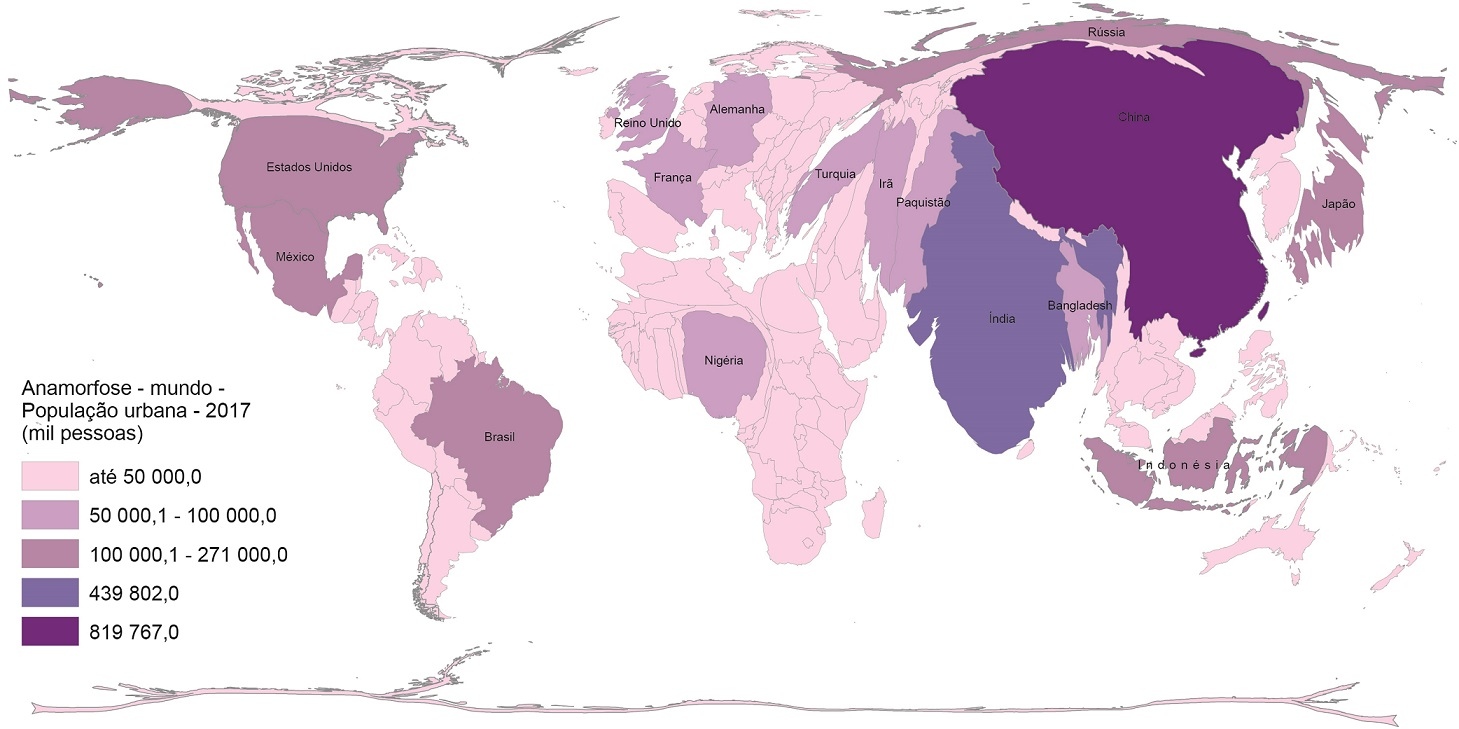
\includegraphics[width=\textwidth]{./imgs/img4.jpg}
\caption{Fonte: https://educa.ibge.gov.br/professores/educa-recursos/20815-anamorfose.html}
\end{figure}

A anamorfose acima está representando

\begin{escolha}
\item
  a produção agrícola.
\item
  a cobertura de nuvens.
\item
  o desenvolvimento humano.
\item
  a quantidade absoluta de população urbana.
\end{escolha}

\coment{SAEB: Contempla ainda o conhecimento necessário para identificação e
compreensão dos diversos elementos que compõem a cartografia.

BNCC: (EF09GE09) Analisar características de países e grupos de países
europeus, asiáticos e da Oceania em seus aspectos populacionais,
urbanos, políticos e econômicos, e discutir suas desigualdades sociais e
econômicas e pressões sobre seus ambientes físico-naturais.

a) Incorreta. Tal alternativa poderia ser correta se o segundo país em
  destaque fosse os Estados Unidos da América e não a Índia. Além disso,
  a Rússia teria um destaque maior;
b) Incorreta. A Antártida e o Brasil seriam áreas destacadas neste caso,
  além das áreas próximas ao Polo Norte;
c) Incorreta: Nesse caso haveria maior correspondência com a Europa,
  Estados Unidos e Oceania;
d) Correta. Os países com as maiores populações urbanas absolutas são
  aqueles mais populosos, caso da Índia e China.}

\num{5}

\begin{quote}
A excelente banda formada por imigrantes indianos radicados no
Reino Unido, conhecida por \textit{Asian Dub Foundation}, vai lançar uma
coletânea retrospectiva com seus maiores sucessos. Time Freeze: 1995 --
2007 The Best Of sai no dia 30 de abril na terra da rainha {[}...{]}.

\fonte{SANCHES, Luciana Maria. 07 mar. 2007. \emph{Omelete}.
Acesso em: 22 fev. 2023.}
\end{quote}

As características da banda citada são exemplos do processo de globalização, pois se caracteriza por

\begin{escolha}
\item
  disputar o mercado cultural britânico.
\item
  evitar o uso comercial de sua produção.
\item
  integrar elementos culturais antes dissociados.
\item
  invisibilizar sua origem através da imigração.
\end{escolha}

\coment{SAEB: Considera o campo instrumental e metodológico da Geografia e da
História, abarcando aprendizagens relativas a categorias como as de
continuidades, mudanças e rupturas, bem como habilidades de
identificação, análise, descrição, comparação e construção de
explicações sobre espaços e tempos em relações multiescalares (local,
regional, nacional e global).

BNCC: (EF09GE05) Analisar fatos e situações para compreender a
integração mundial (econômica, política e cultural), comparando as
diferentes interpretações: globalização e mundialização.

a) Incorreta. Não há no texto uma menção a intencionalidade de uma
  disputa com o mercado cultural, representante da cultura hegemônica;
b) Incorreta. Apesar de não disputar a indústria cultural hegemônica, a
  banda citada faz uso do comércio, fato mostrado no próprio texto, já
  que trata de lançamento de uma coletânea;
c) Correta. O fato de ser uma banda de indianos fundada na Inglaterra
  demonstra a integração cultural gestada pela globalização, pois não se
  trata de simples turistas e sim cidadãos radicados na Inglaterra e que
  produzem cultura a partir de lá, sem deixar de se identificarem como
  indianos;
d) Incorreta. No texto a origem dos membros está em evidência, o que
  desmente essa alternativa.}

\chapter{2. Energia e circuitos produtivos}

\conteudo{Este módulo partiu do entendimento do conceito de energia para embasar
um raciocínio que sintetiza como ocorre o intermédio da relação
sociedade-natureza através de seus circuitos que exploram os recursos
naturais, o mesmo conceito serve de alicerce para a compreensão dos
fenômenos naturais e sua relação com as intervenções humanas na
paisagem.\\
Habilidade BNCC: EF09GE18.}


\colorsec{Habilidades SAEB}

\begin{itemize}
\item Eixo 2 -- Natureza e questões socioambientais.
\end{itemize}

\num{1} Observe os detalhes da imagem abaixo:

\begin{figure}[htpb!]

\includegraphics[width=\textwidth]{./imgs/img5.jpg}
\caption{Fonte: https://pt.wikipedia.org/wiki/Revolu\%C3\%A7\%C3\%A3o\_Industrial\#/media/Ficheiro:Griffiths'\_Guide\_to\_the\_iron\_trade\_of\_Great\_Britain\_an\_elaborate\_review\_of\_the\_iron\_(and)\_coal\_trades\_for\_last\_year,\_addresses\_and\_names\_of\_all\_ironmasters,\_with\_a\_list\_of\_blast\_furnaces,\_iron\_(14761790294).jpg. O "Black Country", em Midlands Ocidentais, Inglaterra, a oeste de Birmingham, nos anos 1870}
\end{figure}


\num{a)} Como podemos relacionar as chaminés a poluição da natureza?

\linhas{3}

\coment{As chaminés emitem fumaça oriunda da queima, a fumaça leva para a
atmosfera substências que podem intoxicar ser humano e animais, além de
emitir gases que modificam o funcionamento da atmosfera, como o gás
carbônico (CO²)}

\num{b)} Circule o tipo de energia utilizada por essas fábricas:

\begin{multicols}{2}
\red{FÓSSIL}

\red{SOLAR}

\blue{HIDRAULICA}

\blue{EÓLICA}

\end{multicols}

\coment{A primeira revolução industrial pautou-se na utilização da queima do
carvão mineral, um combustível fóssil, originado da mineralização de
restos vegetais, a queima dele esquentava água que gerava vapor capaz de
mover máquinas rudimentares.}

\num{2} Na imagem se percebe a existência de elementos rurais ao lado das fábricas.

Sobre esse fato, analise as afirmativas abaixo e marque V para verdadeiro e F para falso.

\begin{boxlist}
\item As cidades industriais intensificaram a transformação da natureza e
do meio rural. \coment{V}

\item O surgimento das indústrias centralizou a economia nas cidades. \coment{V}

\item A presença de fazendas nas cidades exemplifica o convívio duradouro
entre os tipos de produção. \coment{F}

\item A natureza repõe seus recursos mais rápido do que a necessidade
industrial. \coment{F}
\end{boxlist}

\coment{A urbanização praticamente eliminou as atividades rurais dos centros
urbanos, concentrando-as na zona rural. A produção industrial demanda
recursos em uma velocidade superior àquela em que natureza os produz, o
carvão por exemplo leva ao menos 400 milhões e ano para se formar e pode
ser esgotado em algumas décadas.}

\num{3}

\begin{quote}
Apesar de ser usada em vários contextos diferentes, o uso
científico da palavra energia tem um significado bem definido e preciso:
Potencial inato para executar trabalho ou realizar uma ação. Qualquer
coisa que esteja trabalhando, movendo outro objeto ou aquecendo-o, por
exemplo, está gastando (transferindo) energia. {[}...{]}

\fonte{Disponível em:
www.eletronuclear.gov.br/Sociedade-e-Meio-Ambiente/Espaco-do-Conhecimento/Paginas/O-que-e-Energia.
Acesso em: 26 fev. 2023.}
\end{quote}

Cite 3 situações em que ocorre uso de energia em seu cotidiano.

\linhas{2}

\coment{O aluno deve citar quaisquer situações em que ocorra uso de energia,
como atividades físicas (energia metabólica), funcionamento de aparelhos
elétricos e motores.}

\num{4} Para o funcionamento de nosso corpo também precisamos gerar energia,
geramos essa energia a partir dos alimentos que consumimos, como arroz,
feijão, pães de trigo e salada.

Esses alimentos costumam ser cultivados, as plantas também fazem uso de
energia, extraída principalmente da luz solar combinada com os
nutrientes absorvidos do solo.

\begin{figure}[htpb!]
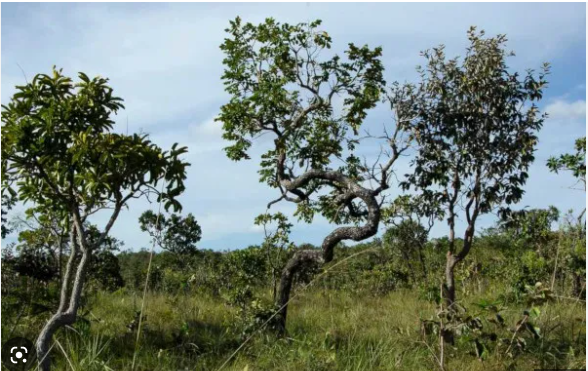
\includegraphics[width=.5\textwidth]{./imgs/img6.png}
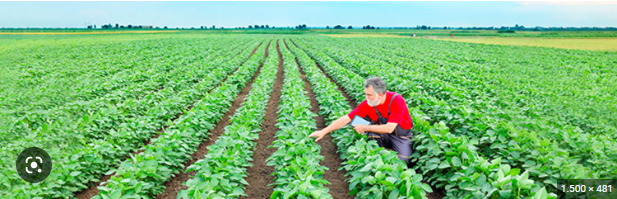
\includegraphics[width=.5\textwidth]{./imgs/img7.png}
\caption{Vegetação natural de Cerrado e Plantio de soja}
\end{figure}

Considerando que sempre existe uma vegetação natural original, é correto
dizer que na imagem II há uma manipulação da energia pelo ser humano?
Justifique.

\linhas{3}

\coment{Sim, pois na primeira imagem, uma formação natural está utilizando a
energia para crescer, já na imagem II ocorreu o plantio de soja que
também vai utilizar a energia solar para crescer, mas de uma maneira
planejada pelo ser humano.}

\num{5} As cidades dependem muito do que vem de fora, desde os alimentos que
são produzidos fora dos limites urbanos e até da própria água, que
muitas vezes é extraída longe da cidade.

Na nuvem de palavras abaixo, pinte aquelas que representam ações capazes
de aproximar a cidade de suas necessidades:

\begin{multicols}{2}
\red{CONSTRUÇÃO DE HORTAS URBANAS}

\red{DRENAGEM TOTAL DE RIOS E PÂNTANOS}

\blue{CRIAÇÃO DE FLORESTAS URBANAS}
\end{multicols}

\coment{A construção de hortas urbanas aproximam a produção de alimentos dos
moradores das cidades, as florestas promovem melhoria geral da qualidade
do ar e ainda garantem a preservação de nascentes, sendo duas ações que
aproximariam as cidades de suas necessidades.}

\num{6} A manutenção natural do calor na atmosfera terrestre é chamada de
efeito estufa, que está representado a seguir:

\begin{figure}[htpb!]

\includegraphics[width=3.07283in,height=3.91428in]{./imgs/img8.png}
\end{figure}

\linhas{2}

\coment{O efeito estuda é a retenção do calor feita pela atmosfera terrestre e
seus componentes, outras respostas aproximadas devem ser consideradas,
já que a base da questão é a imagem.}

\num{6}

\begin{quote}
\textbf{Texto I. O que é Aquecimento Global?}

Aquecimento global é o aumento da temperatura média dos oceanos e
da camada de ar próxima à superfície da Terra {[}...{]} Isto se deve
principalmente ao aumento das emissões de gases na atmosfera que causam
o efeito estufa, principalmente o dióxido de carbono
(CO²).

\fonte{Disponível em:
wwf.org.br/natureza\_brasileira/reducao\_de\_impactos2/clima/mudancas\_climaticas2/.
Acesso em: 26 fev. 2023.}
\end{quote}

\begin{quote}
\textbf{Texto II}

Várias fontes antropogênicas contribuem para as \textbf{emissões
de gases de efeito estufa}. As duas fontes principais são a queima de
combustíveis fósseis e o desmatamento de regiões tropicais como a
Amazônia. A queima de combustíveis fósseis (gás natural, carvão mineral
e, especialmente, petróleo) ocorre principalmente pelo setor de produção
de energia (termelétricas), industrial e de transporte (automóveis,
ônibus, aviões, etc.). {[}...{]} No caso das florestas, as quais
representam um importante estoque natural de carbono, o desmatamento e
as queimadas estão contribuindo para o efeito estufa, uma vez que
liberam o carbono armazenado na biomassa florestal para a atmosfera na
forma de CO².

\fonte{Disponível em:
https://ipam.org.br/entenda/quais-sao-as-principais-fontes-de-gases-de-efeito-estufa-decorrentes-das-atividades-humanas-2/.
Acesso em: 26 fev. 2023.}
\end{quote}

Seria correto afirmar que o aquecimento global é a intensificação do
efeito estufa? Comente.

\linhas{2}

\coment{Sim, no texto I se menciona que o aumento da emissão de gases estufa é a
causa do aquecimento global.}

\num{8} Leia o texto a seguir, repare que algumas palavras estão ausentes:

\begin{quote}
Os últimos 300 anos marcaram uma profunda mudança na relação da
sociedade com a natureza, pois a partir das \salmao{revoluções}
industriais o homem passou a consumir os recursos naturais em uma
velocidade maior em que aquela que a natureza se \salmao{renova.}

Novas necessidades surgiram, e as necessidades do ser humano
passaram a ser todas intermediadas pela indústria e pautadas no
consumismo de produtos que logo são descartados. A necessidade de
produzir mais e mais, necessita utilizar grandes volumes de
\salmao{energia,} obtidos principalmente a partir da queima de
\salmao{combustíveis} fósseis. A queima de \salmao{combutívei}s fósseis
emite gás carbônico que intensifica a retenção de calor na atmosfera,
alterando os \salmao{ciclos} naturais do clima.
\end{quote}

Use as palavras abaixo para completar o texto, uma delas se repete.

\begin{multicols}{2}
\red{RENOVA}

\red{REVOLUÇÕES}

\red{COMBUSTÍVEIS}

\blue{ENERGIA}

\blue{CICLOS}
\end{multicols}

\num{9} O que são Ilhas de Calor?

\begin{quote}
Ilhas de calor é o nome que se dá a um fenômeno climático que
ocorre principalmente nas cidades com elevado grau de urbanização.
Nestas cidades, a temperatura média costuma ser mais elevada do que nas
regiões rurais próximas.

Para entendermos melhor este fenômeno climático, podemos usar como
exemplo a cidade de São Paulo que é considerada uma ilha de calor. Como
esta cidade tem grande concentração de asfalto (ruas, avenidas) e
concreto (prédios, casas e outras construções), ela concentra mais
calor, fazendo com que a temperatura fique acima da média dos municípios
da região. {[}...{]}

\fonte{Disponível em: www.geografia.seed.pr.gov.br/modules/conteudo/conteudo.php?conteudo=244. Acesso em: 28 fev. 2023.}
\end{quote}

Complete a tabela abaixo com duas soluções plausíveis para as causas das ilhas de calor.

\begin{tabular}{l|l}
\hline
\textbf{Causa} & \textbf{Solução} \\ \hline
Excesso de construções & \begin{tabular}[c]{@{}l@{}}\rosa{Melhoria da ventilação natural de prédios e}\\ \rosa{bairros, construção de áreas de lazer abertas,}\\ \rosa{arquitetura verde}\end{tabular} \\ \hline
Ausência de vegetação contínua & \begin{tabular}[c]{@{}l@{}}\rosa{Reflorestamento, arborização urbana,}\\ \rosa{valorização do paisagismo}\end{tabular} \\ \hline
\end{tabular}


\num{10}

\begin{quote}
{[}...{]} Atualmente, a vida útil de um telefone, observa ele,
é de dois anos. Depois disso, é comum que eles comecem a dar problemas e
Muros explica que o reparo pode custar até 40\% do que se gastaria na
compra de um novo. "Se a obsolescência programada não existisse, um
telefone celular teria uma vida útil de 12 a 15 anos", diz. {[}...{]}

\fonte{I. R. Um celular poderia durar 12 anos se sua vida não
fosse encurtada de propósito. \emph{El País}. 15 nov. 2018. Disponível
em: https://brasil.elpais.com/brasil/2018/11/09/tecnologia/1541771036\_210342.html.
Acesso em: 28 fev. 2023.}
\end{quote}

Comente sobre os impactos da obsolescência programada:

\begin{escolha}
\item  Na utilização de energia pelas indústrias.

\linhas{2}

\coment{Como os produtos duram pouco, é preciso que se produza com maior
frequência, gerando mais gasto energético.}

\item  Na exploração de recursos naturais.

\linhas{2}

\coment{A produção precisa suprir a pouca durabilidade dos produtos, extraindo
um volume maior de recursos.}

\item Na vida das pessoas.

\linhas{2}

\coment{Há impacto negativo na vida das pessoas que não conseguem realizar suas
tarefas quando os produtos estragam, além de precisam desembolsar mais
dinheiro para garantir o acesso a itens básicos.}
\end{escolha}

\colorsec{Treino}

\num{1}

\begin{quote}
Que tal você mesmo gerar a energia que consome em casa, a
partir da captação da luz solar? Melhor ainda: que tal vender para a
distribuidora, como a CPFL, por exemplo, a energia excedente? Pois é,
essa realidade tem aumentado substancialmente no Brasil.

Segundo a~Agência Nacional de Energia Elétrica (Aneel), nos
últimos dois anos, a instalação de painéis solares para geração própria
de energia elétrica aumentou mais de 560\%. O número saltou de 7.400
para 49 mil unidades em todo o Brasil. São instalações em residências,
empresas e indústrias.

O que atrai o consumidor, segundo a Aneel, é o preço do
investimento, que tem diminuído ano após ano, e porque há casos em que a
economia de custo desse insumo chega a 95\%.

\fonte{Instalação de painéis solares cresce 560\% no País.
\emph{Jornal da Usp}. 09 dez. 2019. Disponível
em: https://jornal.usp.br/atualidades/instalacao-de-paineis-solares-cresce-560-no-pais/.
Acesso em: 28 fev. 2023.}
\end{quote}

O impacto ambiental do tipo de produção elétrica citado se dá em razão

\begin{escolha}
\item
  do aumento de produção de painéis.
\item
  da eliminação de redes elétricas cabeadas.
\item
  do melhor aproveitamento da energia disponível.
\item
  da diminuição do consumo total de energia elétrica.
\end{escolha}

\coment{SAEB: Trata-se de compreender as razões e os processos pelos quais a
sociedade busca conhecer, explorar e alterar recursos naturais, além de
prever e prevenir catástrofes ambientais por meio da ciência e da
tecnologia.

BNCC: (EF09GE18) Identificar e analisar as cadeias industriais e de
inovação e as consequências dos usos de recursos naturais e das
diferentes fontes de energia (tais como termoelétrica, hidrelétrica,
eólica e nuclear) em diferentes países.

a) Incorreta. Se considerarmos apenas o aumento da produção de painéis,
teríamos um impacto potencialmente negativo em razão da exploração dos
recursos naturais;
b) Incorreta. No texto cita-se que existem aproximadamente 50 000 painéis
solares domésticos, o que é insuficiente para suprir toda a demanda
energética do país que tem mais de 200 milhões de habitantes;
c) Correta. A instalação de painéis solares permite o aproveitamento do
potencial energético local, já que são instalados em cima de casas para
poder captar a energia do Sol;
d) Incorreta. Os painéis não geram diminuição do consumo de energia apenas
se tornam uma fonte a mais de eletricidade disponível.}

\num{2}

\begin{quote}
Para enfrentar o calor que tem passado dos 30ºC, a Prefeitura de
Tietê resolveu pintar as ruas do município, localizado no interior de
São Paulo. A gestão municipal começou a aplicar, sobre o asfalto preto,
uma camada de tinta azul ciano. A técnica vem da área de climatologia e
é capaz de trazer bons resultados.

"A cor azul ciano reduz a temperatura em 10\% e auxilia na economia de
energia elétrica e na redução da evaporação, o que torna o ambiente mais
fresco para pessoas, plantas e animais", justifica a Prefeitura. A
gestão afirma que o gasto com a tinta será compensado pela possível
redução de consumo de energia elétrica pela população.

{[}...{]}

\fonte{Para atenuar calor, prefeitura pinta asfalto de azul.
\emph{Estadão Conteúdo.} 21 jan. 2019. Disponível em:
www.otempo.com.br/interessa/saude-e-ciencia/para-atenuar-calor-prefeitura-pinta-asfalto-de-azul-1.2124802.
Acesso em: 28 fev. 2023.}
\end{quote}

Uma solução efetiva para o melhor conforto térmico seria a criação de estruturas espaciais capazes de desempenhar

\begin{escolha}
\item
  armazenamento da chuva.
\item
  concentração do aquecimento solar.
\item
  aquecimento da parte superior de construções.
\item
  absorção da energia solar através de fotossíntese.
\end{escolha}

\coment{SAEB: Além de abarcar a compreensão da dinâmica dos fenômenos naturais,
propõe a superação da dicotomia entre natureza e sociedade e a reflexão
sobre as formas de intervenção humana em diferentes tempos e espaços.

BNCC: (EF09GE18) Identificar e analisar as cadeias industriais e de
inovação e as consequências dos usos de recursos naturais e das diferentes fontes de energia (tais
como termoelétrica, hidrelétrica, eólica e nuclear) em diferentes países.

a) Incorreta. Armazenamento da chuva não tem capacidade de redução da
temperatura atmosférica;
b) Incorreta. Tal ação aumentaria calor atmosférico, fenômenos urbanos como
as ilhas de calor concentram o aquecimento solar nas cidades aumentando
a temperatura;
c) Incorreta. O aquecimento da parte superior gera a retenção dê calor no
interior das construções;
d) Correta. A energia solar disponível será utilizada sempre de alguma
forma, quando você tem muitas construções elas absorvem o calor solar
emitindo o de volta para a atmosfera, gerando aquecimento, enquanto que
em uma área densamente vegetada, a energia solar é absorvida pelas
plantas que a transformam em energia metabólica.}

\num{3}

\begin{quote}
As mudanças climáticas antropogênicas, ou seja, aquelas causadas
pelo homem, estão associadas ao aumento da emissão de gases de efeito
estufa por queima de combustíveis fósseis (dos automóveis, das
indústrias, usinas termoelétricas), queimadas, desmatamento,
decomposição de lixo etc. A partir do final do século 18 (Revolução
Industrial) e na segunda metade do século 20, houve uma expansão da
produção industrial, o que gerou um grande aumento de emissões de gases
de efeito estufa na atmosfera. Existem fortes indícios de que o clima
está de fato mudando. As décadas de 1990 e 2000 foram as mais quentes
dos últimos 1.000 anos. As projeções do Painel Intergovernamental de
Mudanças Climáticas (IPCC) indicam que nos próximos 100 anos poderá
haver um aumento da temperatura média global entre 1,8°C e 4,0°C, e um
aumento do nível médio do mar entre 0,18 m e 0,59 m, o que pode afetar
significativamente as atividades humanas e os ecossistemas terrestres.

\fonte{Disponível em: www.inpe.br/faq/index.php?pai=9\#:~:text=A\%20partir\%20do\%20final\%20do,clima\%20est\%C3\%A1\%20de\%20fato\%20mudando. Acesso em: 28 fev. 2023.}
\end{quote}

A relação entre gases estufa e mudanças climáticas é explicada pelo fato
de as emissões humanas passarem a compor

\begin{escolha}
\item
  uma interferência dissociada dos ciclos naturais.
\item
  a capacidade de resfriamento atmosférico.
\item
  o ciclo de crescimento florestal.
\item
  o sistema climático global.
\end{escolha}

\coment{SAEB: Trata-se de compreender as razões e os processos pelos quais a
sociedade busca conhecer, explorar e alterar recursos naturais, além de
prever e prevenir catástrofes ambientais por meio da ciência e da
tecnologia.

BNCC: (EF09GE18) Identificar e analisar as cadeias industriais e de
inovação e as consequências dos usos de recursos naturais e das diferentes fontes de energia (tais
como termoelétrica, hidrelétrica, eólica e nuclear) em diferentes países.

a) Incorreta. O fato de as emissões humanas estarem interferindo no clima
global, mostram que há uma integração da sociedade com o ciclo climático
global;
b) Incorreta. Os gases do efeito estufa não tem capacidade de gerar
resfriamento atmosférico;
c) Incorreta. Apesar de poderem favorecer crescimento Florestal, as
emissões de gases do efeito estufa tem seu maior impacto no aquecimento
atmosférico, estando também relacionada a própria destruição Florestal
existente, já que o desmatamento promove a emissão de gás carbônico;
d) Correta. As emissões de gases do efeito estufa sem integraram a dinâmica
climática, pois o maior aquecimento atmosférico está alterando os ciclos
dos sistemas atmosféricos e terrestres como um todo.}


\chapter{Simulado}

\num{1}

\begin{quote}
Carvão é o nome dado a diversas rochas sedimentares passíveis
de uso como combustível, constituídas de um material heterogêneo
originado de restos vegetais depositados em águas rasas, protegidos da
ação do oxigênio do ar. {[}...{]}

A extração do carvão pode ser em minas a céu aberto ou
subterrâneas, dependendo da profundidade em que se encontra a camada. As
minas a céu aberto exercem significativo impacto ambiental em razão dos
elementos químicos contidos no carvão, como o enxofre.

Numerosas áreas de mineração antigas no sul do Brasil, trabalhadas
em uma época em que a preocupação com o ambiente natural era muito menor
que atualmente, foram muito degradadas e precisaram ser recuperadas,
trabalho que vem sendo feito nas últimas décadas.

\fonte{Disponível em:
http://www.cprm.gov.br/publique/SGB-Divulga/Canal-Escola/Carvao-Mineral-2558.html.
Acesso em: 28 fev. 2023.}
\end{quote}

É possível identificar que o principal impacto da extração de carvão se dá

\begin{escolha}
\item
  pela emissão local de fumaça.
\item
  pela geração de ilhas de calor.
\item
  pela exaustão do lençol freático.
\item
  pela remoção da estrutura superficial do solo.
\end{escolha}

\coment{SAEB: Trata-se de compreender as razões e os processos pelos quais a
sociedade busca conhecer, explorar e alterar recursos naturais, além de
prever e prevenir catástrofes ambientais por meio da ciência e da
tecnologia.

BNCC: (EF09GE18) Identificar e analisar as cadeias industriais e de
inovação e as consequências dos usos de recursos naturais e das diferentes fontes de energia (tais como termoelétrica, hidrelétrica, eólica e nuclear) em diferentes países.

a) Incorreta. A extração do carvão não produz massiva emissão de fumaça;
b) Incorreta. As ilhas de calor são fenômenos associados a grandes
  cidades;
c) Incorreta. Ao contrário da mineração de metais, não se utiliza água
  para a extração de carvão mineral;
d) Correta. Para extrair o carvão toda a superfície acima da mina precisa
  ser removida, assim, o solo é cobertura vegetal são despertados.}

\num{2}

\begin{figure}[htpb!]
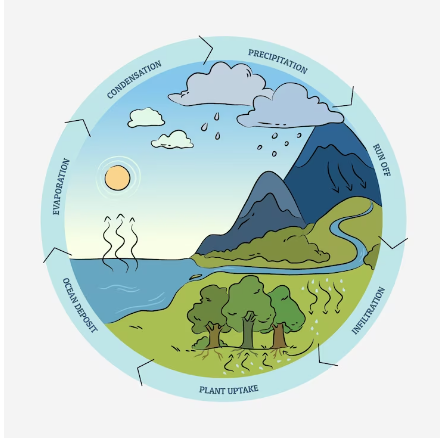
\includegraphics[width=4.58333in,height=4.56250in]{./imgs/img9.png}
\caption{Fonte:
https://br.freepik.com/vetores-gratis/informacoes-desenhadas-a-mao-sobre-o-ciclo-da-agua\_18980469.htm\#query=ciclo\%20da\%20agua\&position=1\&from\_view=keyword\&track=ais.}
\end{figure}

Analisando a imagem é correto dizer que a absorção de energia ocorre

\begin{escolha}
\item
  No escoamento.
\item
  Na precipitação.
\item
  Na condensação.
\item
  Na evaporação.
\end{escolha}

\coment{SAEB: Além de abarcar a compreensão da dinâmica dos fenômenos naturais,
propõe a superação da dicotomia entre natureza e sociedade e a reflexão
sobre as formas de intervenção humana em diferentes tempos e espaços.

BNCC: (EF09GE18) Identificar e analisar as cadeias industriais e de
inovação e as consequências dos usos de recursos naturais e das diferentes fontes de energia (tais como termoelétrica, hidrelétrica, eólica e nuclear) em diferentes países.

a) Incorreta. O escoamento orientado pela força da gravidade e não da
  energia solar;
b) Incorreta. A precipitação é o efeito da perda de calor por parte das
  nuvens, pois ao perder calor o vapor de água condensa se em pequenas
  gotículas formando nuvens e posteriormente chuva;
c) Incorreta. Ao perder calor o vapor de água condensa se em pequenas
  gotículas formando nuvens e posteriormente chuva;
d) Correta. A evaporação é o efeito do ganho de calor por parte da água
  líquida, o que gera sua evaporação, ganho de calor obtido através da
  absorção da energia solar.}

\num{3}

\begin{quote}
{[}...{]}

Três semanas após o terremoto que destruiu partes do sudeste da
Turquia e do noroeste da Síria, e que deixou mais de 50 mil mortos nos
dois países, um novo tremor, de magnitude 5,6, atingiu o território
turco nesta segunda-feira (27), matando uma pessoa e deixando dezenas de
feridos. {[}...{]}

O tremor desta segunda-feira acontece com a região central da
Turquia ainda praticamente sob escombros e tentando achar um caminho
para a reconstrução de cidades inteiras. Mais de 173 mil prédios foram
total ou parcialmente destruídos no país, segundo o governo.

\fonte{Novo terremoto atinge a Turquia, derruba prédios e deixa
um morto e dezenas de feridos. \emph{Estadão Conteúdo}. 27 fev. 2023.
Disponível
em: https://gauchazh.clicrbs.com.br/mundo/noticia/2023/02/novo-terremoto-atinge-a-turquia-derruba-predios-e-deixa-um-morto-e-dezenas-de-feridos-clemqhxqs005301e9uleel18t.html.
Acesso em: 28 fev. 2023.}
\end{quote}

Tamanha destruição estrutural poderia ser evitada caso ocorresse a (o)

\begin{escolha}
\item
  produção de estruturas físicas mais resistentes aos tremores.
\item
  transferência de cidades para áreas próximas mais planas.
\item
  previsão antecipada de tremores de terra.
\item
  mapeamento de rotas de fuga.
\end{escolha}

\coment{SAEB: Além de abarcar a compreensão da dinâmica dos fenômenos naturais,
propõe a superação da dicotomia entre natureza e sociedade e a reflexão
sobre as formas de intervenção humana em diferentes tempos e espaços.

BNCC: (EF09GE18) Identificar e analisar as cadeias industriais e de
inovação e as consequências dos usos de recursos naturais e das
diferentes fontes de energia (tais como termoelétrica, hidrelétrica,
eólica e nuclear) em diferentes países.

a) Correta. Especialistas apontaram que a falta de adequação das estruturas
foi uma das causas da grande destruição ocorrida;
b) Incorreta. O tectonismo não varia a sua atividade em razão do terreno e
sim da distância em relação às ao limite de placas ou falhamentos;
c) Incorreta. Não é possível prever com exatidão a ocorrência de
terremotos;
d) Incorreta. Como terremotos são eventos generalizados rotas de fuga são
elementos muito paliativos, sendo adequação das estruturas parte
fundamental dos esforços para evitar tragédias como a citada.}

\num{4}

\begin{quote}
{[}...{]}

Carlos Nobre afirma que há mais de 50 produtos derivados do açaí,
mas que não foram desenvolvidos na Amazônia. O bioma produz inúmeros
produtos primários, como açaí, castanha e cacau, que passam no máximo
por um pré-processamento naquela região. ``A maior parte dos produtos
derivados do açaí foram desenvolvidos nos Estados Unidos. A indústria de
transformação é praticamente inexistente na Amazônia, mas o potencial
dos produtos da biodiversidade é gigantesco. Não casamos esse potencial
do aproveitamento da biodiversidade com a indústria'', diz. De acordo
com o conceito lançado por Nobre, o açaí, que é um alimento base das
populações interioranas da Amazônia, pode provocar o desenvolvimento
sustentável daquela região, criando milhares de empregos e, ao mesmo
tempo, promovendo a conservação do meio ambiente. {[}...{]}

\fonte{FONSECA, Eliane. \emph{Portal Unicamp}. Disponível em:
https://ige.unicamp.br/news/2019-10/carlos-nobre-apresenta-o-conceito-da-terceira-viaamazonia-40.
Acesso em: 28 fev. 2023.}
\end{quote}

Carlos Nobre defende que a destruição da Amazônia pode ser combatida através da aplicação de

\begin{escolha}
\item
  derrubada florestal.
\item
  remoção das populações.
\item
  restrições da atividade econômica.
\item
  processamento industrial de produtos florestais.
\end{escolha}

\coment{SAEB: Trata-se de compreender as razões e os processos pelos quais a
sociedade busca conhecer, explorar e alterar recursos naturais, além de
prever e prevenir catástrofes ambientais por meio da ciência e da
tecnologia.

BNCC: (EF09GE18) Identificar e analisar as cadeias industriais e de
inovação e as consequências dos usos de recursos naturais e das diferentes fontes de energia (tais como termoelétrica, hidrelétrica, eólica e nuclear) em diferentes países.

a) Incorreta. No texto ele critica a lógica econômica baseada na destruição
ambiental;
b) Incorreta. Não há no texto nenhuma indicação para remoção de populações,
pelo contrário, se discute como criar novas oportunidades econômicas
para a população;
c) Incorreta. o texto discute exatamente a ampliação das atividades
econômicas e não sua restrição;
d) Correta. No texto há menção ao desenvolvimento de produtos e a
necessidade de associar a indústria aos produtos amazônicos, propondo
que o desenvolvimento industrial baseado em produtos típicos seja uma
das soluções para o desenvolvimento sustentável.}

\num{5}

\begin{quote}
Essa é uma entre tantas consequências da globalização: um número
reduzido de empresas multinacionais controla uma parte importante do
mercado mundial de alimentos.

O resultado é que tais firmas concentram uma enorme influência para
determinar como a comida é repartida no mundo. Potencialmente, também
têm a capacidade de determinar ações que podem ajudar a aliviar a fome
no planeta {[}...{]}

Esas empresas operam em mercados globais em que a produção de alguns
itens está concentrada em poucas empresas.

Irit Tamir aponta como exemplo três delas, que atuam na cadeia de valor
do cacau {[}...{]} . Elas controlam 40\% do comércio mundial nessa área.
{[}..{]}

\fonte{AFP. As dez multinacionais que controlam o mercado
mundial de alimentos. \emph{BBC Brasil}. 30 out. 2016. Disponível em:
www.bbc.com/portuguese/geral-37710637.
Acesso em: 28 fev. 2023.}
\end{quote}

É possível diminuir o monopólio de poucas empresas sobre a produção
alimentar através do desenvolvimento de

\begin{escolha}
\item
  circuitos regionais de produção alimentar.
\item
  conglomerados nacionais de produção agrícola.
\item
  mercados favoráveis aos conglomerados internacionais.
\item
  sistemas alimentares baseados em monoculturas de cereais.
\end{escolha}

\coment{SAEB: Por conseguinte, o eixo avança na reflexão sobre as questões
ambientais, notadamente aquelas decorrentes da interação
natureza-sociedade, passando por questões como sustentabilidade,
segurança alimentar, posicionamentos de instituições e países e o
próprio ambientalismo e suas variações.

BNCC: (EF09GE18) Identificar e analisar as cadeias industriais e de
inovação e as consequências dos usos de recursos naturais e das diferentes fontes de energia (tais como termoelétrica, hidrelétrica, eólica e nuclear) em diferentes países.

a) Correta. Tal ação permitiria a promoção dos cultivos locais, sua
  respectiva venda e aproveitamento industrial, já que um circuito
  constitui todo um sistema articulado de produção, um exemplo são as
  regiões vinícolas sulistas ou mesmo leiteiras de Minas Gerais;
b) Incorreta. Os conglomerados estão sujeitos a mesma lógica das grandes
  empresas alimentares, nesse sentido, concentrar a produção alimentar
  não atingiria o objetivo solicitado pela questão;
c) Incorreta. Tal ação beneficiaria a venda dos produtos oriundos dos
  monopólios, assim não atingiria o objetivo solicitado pela questão;
d) Incorreta. As monoculturas são a base sob a qual os monopólios
  alimentares se sustentam, pois estão diretamente associados ao
  processamento de cultivos de larga escala como arroz, soja, trigo,
  oleaginosas e carne.}


